\subsection{Materials}

\subsubsection{Databases}

For OD detection, since the operation must be effective in many different clinical cases, the proposed method was evaluated on ten databases among the most popular public databases in retinal image study. In particular, they were developed to detect various ocular pathologies, test a diagnosis protocol or extract retinal structures, and were used in both medical or even non-medical contexts.
VARIA \citep{varia,varia2} database contains 58 gray-scale images, used for the authentication of individuals via the vascular tree. DRIVE database \citep{drive} consists of 40 retinal images, and was developed for the segmentation of the retinal vascular tree. The STARE project \citep{stare,stare2}, mainly used to detect the OD, established a 81-images database with 31 healthy images and 50 pathological ones. MESSIDOR \citep{messidor} was created for diabetic retinopathy screening, with its 400 images. HRF database (High-Resolution Fundus) \citep {hrf} with 45 images was established for diabetic retinopathy and glaucoma screening. ROC database \citep{roc}, created for micro-aneurysms detection linked to diabetic retinopathy, is composed of 50 images. DIARETDB0 \citep{diaretdb0} and DIARETDB1 \citep{diaretdb1} were also developed for the detection of diabetic retinopathy. These databases include 130 and 89 retinal images respectively. 
Finally, the E-OPHTHA-EX and E-OPHTHA-MA databases \citep{eophtha}, respectively composed of 82 and 124 images, were mainly developed to detect different types of lesions caused by diabetic retinopathy (exudates, micro-aneurysms).
\bigbreak
For OC and OD segmentation, and final glaucoma screening, the validation stage was conducted with the same database. 
%Regarding to a few relevant works for glaucoma screening using 2-D retinal images \citep{chakravarty}. 
The experiment was performed with the DRISHTI-GS1 database \citep{sivaswamy2014drishti, drishti}, which consists of 51 retinal color images, captured with a 30-degree FOV with a resolution of 2896 x 1944. 
%The database was built with healthy subjects and subjects suffering from glaucoma only. Hence, no bright lesions related to other ocular diseases such as diabetic retinopathy are apparent. However, the prior method for OD detection is useful when glaucoma screening is operated to subjects eventually suffering from other ocular diseases, to effectively detect the ONH when bright lesions are apparent within the retina. Hence, assessment of the ONH variations and glaucoma screening are reliably performed.
For each captured image of the database, the ground-truth segmentation from four trained experts is provided for the OC and OD areas. The manual markings are computed in a soft map $S$, as the four segmentation results from each respective expert are superimposed in $S$. In our study, a preprocessing step was performed to obtain a three-expert majority consensus on the final ground-truth segmentation \citep{drishti}. This choice allows a good balance between a better unification of all clinical results, and a restricted but precise ground-truth area.

Moreover, for each retinal image from the database, the ground-truth glaucoma diagnosis by the four experts is also provided, with 18 healthy and 32 glaucomatous images. This final diagnosis by experts allows the validation of our glaucoma screening study and obtained results. Here, we use the group majority opinion with at least three out of four experts gives the final diagnosis, as the presence of a healthy or glaucomatous subject.

\subsubsection{\label{metrics3}Evaluation metrics}

For the experimental phase, we introduced several metrics to measure the performance of the proposed method. We exploit often-used metrics related to each stage of the algorithm (OD detection, OC and OD segmentation and glaucoma screening).

For OD detection, the performance is evaluated with the precision metric only. Here, a simple evaluation protocol is followed, as the OD detection point is considered correct if the point is inside the OD region, including its borders. Otherwise, the detection is considered wrong.

On the remainder of this experimental phase, the OC and OD segmentation and the glaucoma screening are assimilated to binary classification tasks. True positives (TP) gather all correctly-classified positive samples. Likewise, true negatives (TN) group all correctly-classified negative samples. Inversely, false positives (FP) gather the actual negative samples classified as positives, and false negatives (FN) gather the actual positive samples classified as negatives.

For the OC and OD segmentation, TP consist of all pixels correctly classified as part of the area, and TN gather all pixels correctly classified as non-part of the segmented area. Inversely, FP gather all pixels labeled as part of the segmented area, when they actually do not be part of the ground-truth manual marking. FN gather the pixels labeled as non-part of the segmented area, when they are actually part of the ground-truth manual marking.

\bigbreak

To evaluate the segmentation step, we compute three metrics \citep{drishti}:

- Sensitivity, also called recall, denotes the proportion of correctly-classified positive pixels among the actual positive pixels:

\begin{equation}
Sen = \frac{TP}{TP+FN}
\label{sensitivity}
\end{equation}

\bigbreak

- The positive predictive value (PPV), also called precision, denotes the proportion of correctly-classified pixels among the labeled-positive pixels:

\begin{equation}
PPV = \frac{TP}{TP+FP}
\label{PPV}
\end{equation}

\bigbreak

- The F-score is a harmonic mean of sensitivity and PPV metrics:

\begin{equation}
F-score = 2 \cdot \frac{Sen \cdot PPV}{Sen + PPV}
\label{fscore}
\end{equation}

\vspace{0.5cm}

For glaucoma screening and diagnosis, the same classification protocol is followed. TP define the subjects correctly diagnosed as glaucomatous. Likewise, TN gather the subjects correctly diagnosed as healthy. Inversely, FP represent the subjects diagnosed as glaucomatous, when they actually do not suffer from glaucoma. This type of error mainly causes a false alarm, with a potential unnecessary treatment. Even worse, the FN represent the subjects suffering from glaucoma, when they are detected as healthy by the glaucoma screening system. This second type of error causes more serious consequences, as the disease is not screened and a treatment at the earlier stage cannot be provided. The detection of the disease presence will occur at further stages, inducing a more expensive and inconvenient treatment. In this way, as an effective detection of potential glaucomatous subject is primordial, a non-healthy subject screening system at the cutting-edge is required. A maximum certainty on the positive labelling is expected.

In this direction, we compute the three metrics in Eq. (\ref{sensitivity}), (\ref{PPV}) and (\ref{fscore}). For glaucoma screening, sensitivity denotes the proportion of correctly-classified glaucomatous subjects among all actual glaucomatous subjects.
PPV denotes the proportion of subjects correctly labeled glaucomatous among the labeled-glaucomatous ones. F-score is a harmonic mean of sensitivity and PPV metrics.

We also compute the three following metrics:

- Specificity (Spe) is the proportion of correctly-classified healthy subjects among all actual healthy subjects:

\begin{equation}
Spe = \frac{TN}{TN+FP}
\label{specificity}
\end{equation}

\bigbreak

- The negative predictive value (NPV) denotes the proportion of correctly-classified healthy subjects among the labeled-healthy ones:

\begin{equation}
NPV = \frac{TN}{TN+FN}
\label{NPV}
\end{equation}

\bigbreak

- Finally, the overall accuracy (Acc) is the proportion of correctly-classified subjects among all subjects (healthy or glaucomatous):

\begin{equation}
Acc = \frac{TP+TN}{TP+TN+FP+FN}
\label{accuracy}
\end{equation}

\bigbreak

These metrics are used to evaluate the glaucoma screening method, by comparing each found diagnosis (healthy or glaucomatous) to the diagnosis from the trained specialists. Hence, in the medical context, these metrics can be interpreted by a ophthalmologist, to assess the usefulness of the system on the final diagnosis \citep{saunders}.
The results obtained on each evaluation metric are expressed in the following section.

\subsection{Results}

\subsubsection{Computation efficiency}

In this section, the time complexity of the proposed method for glaucoma screening is laid out. A summary can be found in \mbox{Table \ref{complexity}}. As noticed in the previous sections (see \mbox{sections \ref{intro}, \ref{related_work}}), one of the main challenges in this work is to propose a computationally-efficient method for glaucoma screening and diagnosis. A further goal is to deploy computer-aided mobile systems, spreading the access to eye health.

We firstly proposed a new method for OD detection \textcolor{blue}{\mbox{(see Algorithm~\ref{alg:oddetection})}}. A prior rigorous study of the existing methods have been conducted. In the presented method, we exploited the brightness feature of the OD \mbox{(see Algorithm~\ref{alg:detectbrightregions})} and a template matching technique \mbox{(see Algorithm~\ref{alg:templatematching})} to detect the OD even in the presence of lesions. 
The detection of the bright regions involves the computation of well-used computer vision algorithms such as Otsu's thresholding, Euclidean distance transform or the extraction of maximum values. Considering $L$ different gray levels in the image, Otsu's thresholding involves in the worst case $\mathcal{O}(L^2)$ operations. Considering a retinal image $I$ with a $n \times n$ size, the distance transform generates a $\mathcal{O}(n^2)$ complexity. Extracting max values in a $n$-length list involves a $\mathcal{O}(n)$ linear research in the worst case. Template matching involves the use of less costing algorithms, since the histogram calculation, the creation of the histogram templates and the matching using cross-correlation generate $\mathcal{O}(1)$ constant or $\mathcal{O}(n)$ linear time complexity. It is important to notice that template matching is applied on a few candidates and not along the whole image, inducing less operations.
As a major advantage, the method avoids the extraction of the vascular tree to effectively detect the OD, often relying on $\mathcal{O}(n^3)$ cubic complexity algorithms \citep{sayadia2}.

Secondly, for OC and OD segmentation \mbox{(see Algorithm~\ref{alg:ocodsegmentation})}, a previous study of the existing methods conducts to propose an unsupervised segmentation method. Here, we used a K-means clustering approach, exploiting the intensity criterion to classify the pixels to each retinal area \mbox{(see Algorithm~\ref{alg:ocodsegmentation}, line \ref{kmeansoperation})}. The main advantage of the K-means clustering is its quick convergence to the final clustering. Also, setting only two parameters (distance $D$, number of clusters $K$) allows quite ease. Despite the K-means clustering is a $\mathcal{O}(KDn^2)$ polynomial algorithm (with $n \times n$ the number of observations to classify) \citep{Xu2015}, it remains one of the computationally-efficient clustering approaches, in comparison with the fuzzy c-means clustering for instance \citep{ghosh}. In practice, with our small OD sub-images, K-means clustering is operated in real-time. A lot of works have improved the K-means clustering complexity, particularly by proposing an efficient initialization of the cluster centers \citep{celebi}. Its practical convenience permits to converge toward a precise segmentation of the areas in an efficient manner. 

To improve the segmentation accuracy, we have employed the circular Hough transform to fit on the boundaries \mbox{(see Algorithm~\ref{alg:ocodsegmentation}, line \ref{houghoperation})}. Circular Hough transform have been extensively used over the decades for pattern recognition purpose \citep{mukhopadhyay}. Recent studies have performed the Hough transform in real-time \citep{weiss}, and a lot of works have studied the Hough transform for an efficient implementation reducing its computational requirements \citep{houghsurvey, soltany2011fast} with $\mathcal{O}(n^2)$-complex algorithms. However, the complexity of the circular Hough transform can rapidly increase with the number of computed circles with different radius for each edge point of the image. Thus, to decrease the computational cost when computing the Hough transform, we restrict the search interval. For that we fix the \mbox{radius $R$} of the final circle in a well-defined interval. Here, we define the \mbox{interval $I_R$ as:}

\begin{equation}
I_R = \Bigg[\frac{R_{area}}{2}; \quad R_{area} + \frac{R_{area}}{2} \Bigg]
\end{equation}

\noindent where $R_{area}$ corresponds respectively to the OC and OD radius approximations, as $R_{OD}$ is defined in \mbox{Eq. (\ref{rayon_disque})} and \mbox{$R_{OC} \approx R_{OD}/2$}. Hence, the circular Hough transform is performed with a few numbers of candidate circles.

Thirdly, for CDR calculation and glaucoma screening \mbox{(see Algorithm~\ref{alg:glaucomascreening})}, simple techniques such as the ratio calculation, and thresholding to classify healthy and glaucomatous subjects rely on $\mathcal{O}(1)$ constant time complexity. The prior calculation of the areas of the OC and OD regions relies on $\mathcal{O}(n^2)$ operations in the worst case.
Finally, the full method for glaucoma screening relies on low-complex algorithms, with a $\mathcal{O}(n^2)$ order of $n^2$ total time complexity, in line with the expressed requirements for a prospective implementation on mobile devices.

\vspace{0.2cm}

\begin{table}[h]
	\begin{center}
		\small
		
		\renewcommand{\arraystretch}{1}
	
		\begin{tabular}{c c c}
			\hline 
			Functions & Parameters & Time complexity \\
			\hline
			Otsu'thresholding & Number of gray levels $L$ & $\mathcal{O}(L^2)$ \\
			Euclidean distance transform & Size of the image $N$ & $\mathcal{O}(N^2)$ \\
			Extract values (max) & length of the list $l$ & $\mathcal{O}(l)$ \\
			Template Matching & Number of histogram bins $H$ & $\mathcal{O}(H^2)$ \\
			
			K-means clustering & Size of the crop $m$, number of clusters $K$, distance $D$ & $\mathcal{O}(KDm^2)$ \\
			Circular Hough Transform & Size of the crop $m$ & $\mathcal{O}(m^2)$ \\
			
			\hline
			
		\end{tabular}
		
	\end{center}
	\caption{\label{complexity}Overview of the worst-case time complexity of the computed functions for glaucoma screening.}
\end{table}

\subsubsection{OD detection and ROI extraction}

\begin{figure*}[t]
    \centering
    
    \begin{tabular}{c c c c}
    	
    	{(1)} &
    	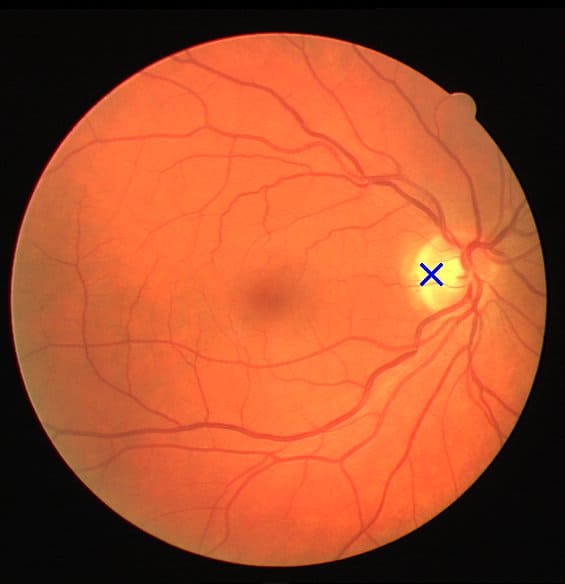
\includegraphics[width=3.0cm]{Images/Methode/Detection/Drive/02_test.jpg}{(a)} & 
    	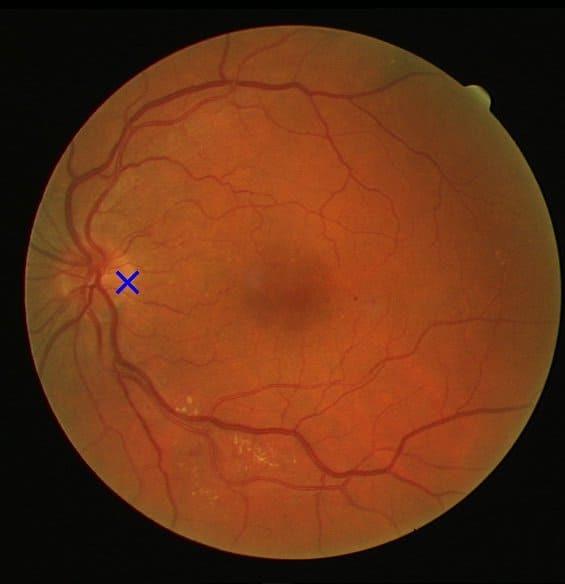
\includegraphics[width=3.0cm]{Images/Methode/Detection/Drive/03_test.jpg}{(b)} &
    	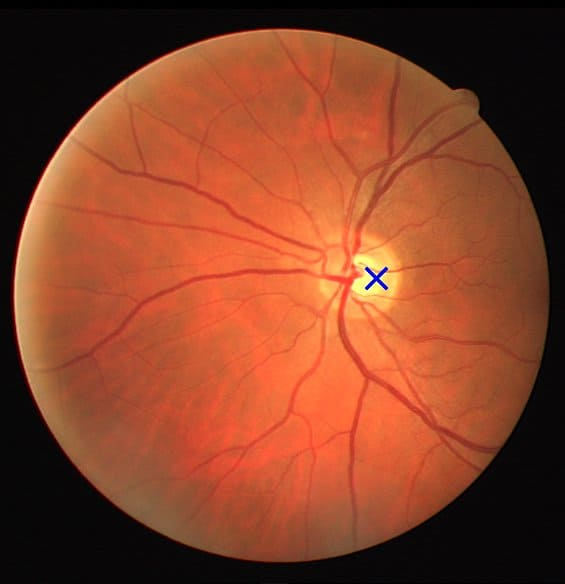
\includegraphics[width=3.0cm]{Images/Methode/Detection/Drive/04_test.jpg}{(c)} \\
    	
    	{} &
    	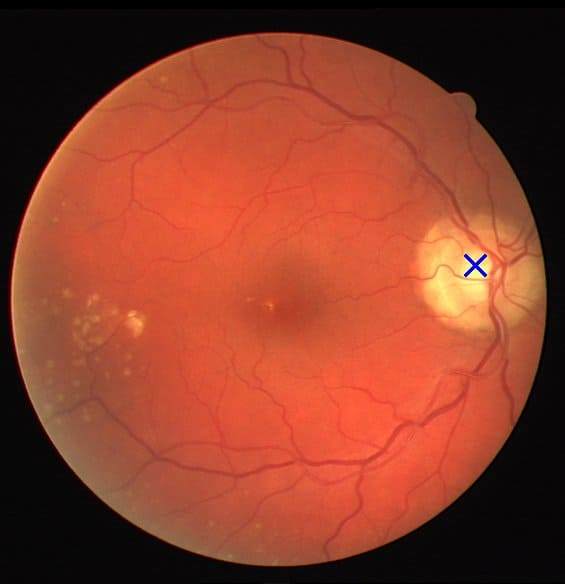
\includegraphics[width=3.0cm]{Images/Methode/Detection/Drive/08_test.jpg}{(d)} & 
    	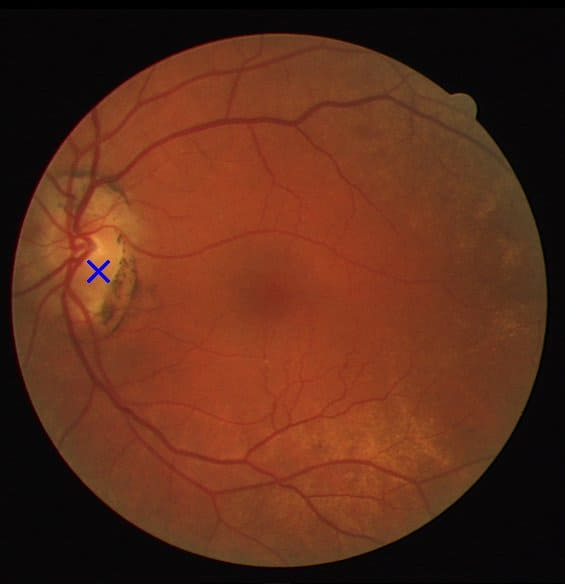
\includegraphics[width=3.0cm]{Images/Methode/Detection/Drive/26_training.jpg}{(e)} &
    	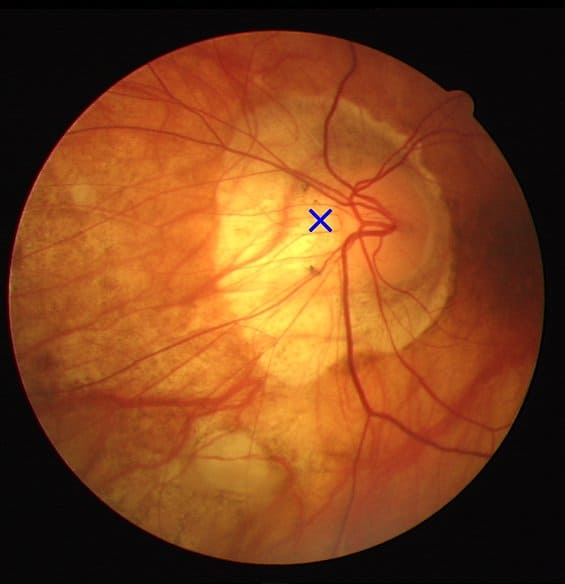
\includegraphics[width=3.0cm]{Images/Methode/Detection/Drive/34_training.jpg}{(f)} \\
    	
    	{(2)} &
    	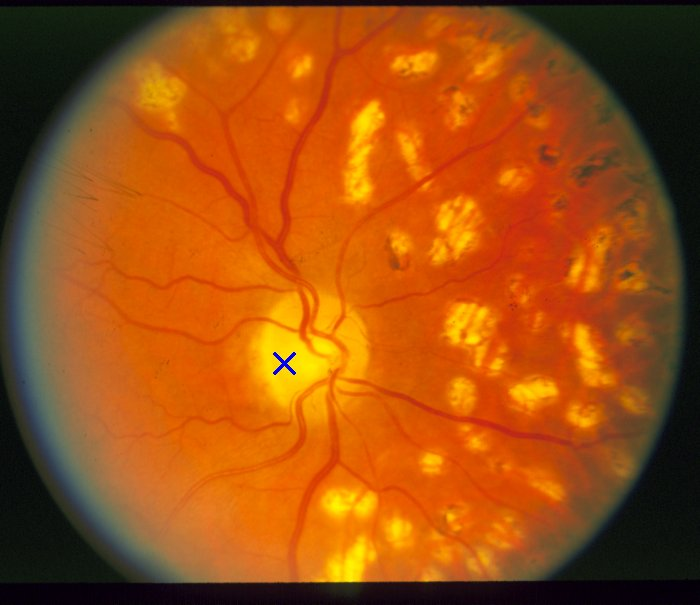
\includegraphics[width=3.0cm]{Images/Methode/Detection/Stare/im0179.jpg}{(g)} & 
    	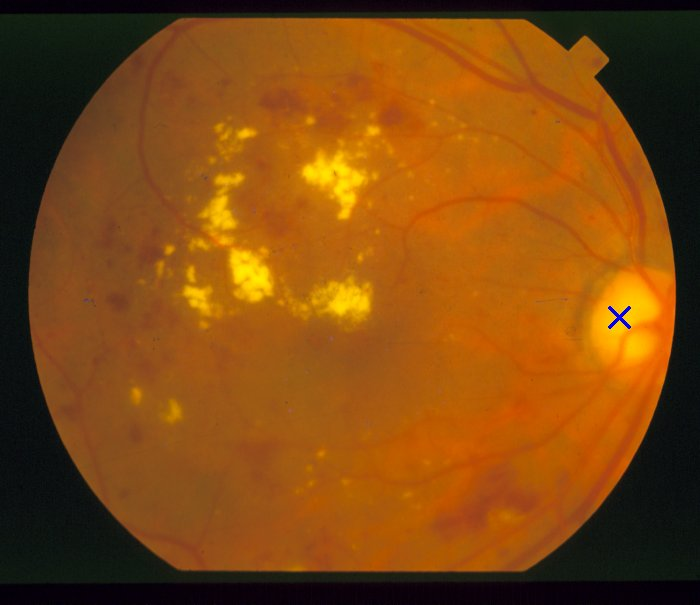
\includegraphics[width=3.0cm]{Images/Methode/Detection/Stare/im0096.jpg}{(h)} &
    	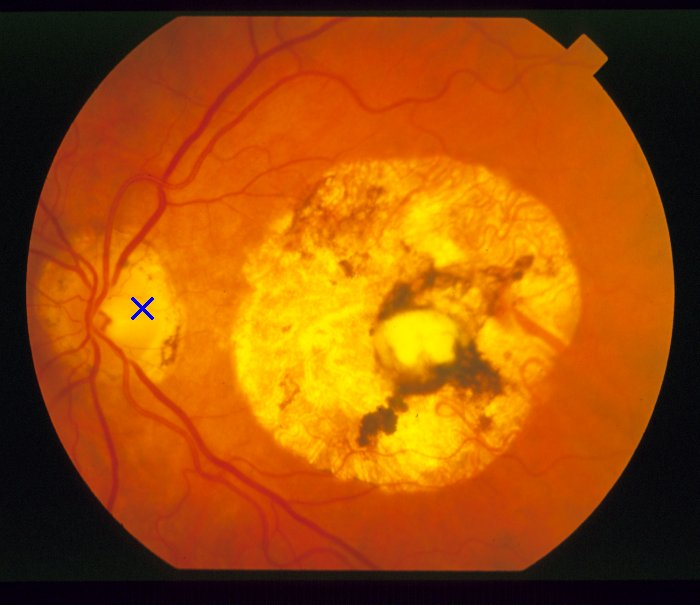
\includegraphics[width=3.0cm]{Images/Methode/Detection/Stare/im0110.jpg}{(i)} \\
    	
    	{} &
    	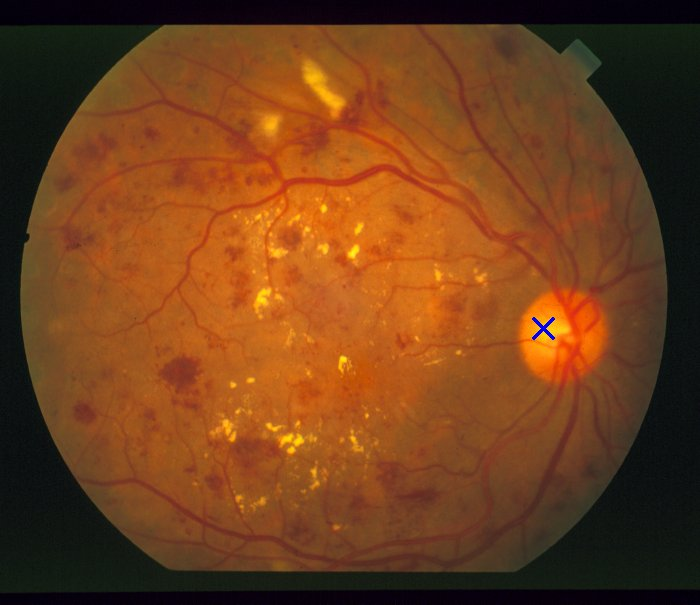
\includegraphics[width=3.0cm]{Images/Methode/Detection/Stare/im0140.jpg}{(j)} & 
    	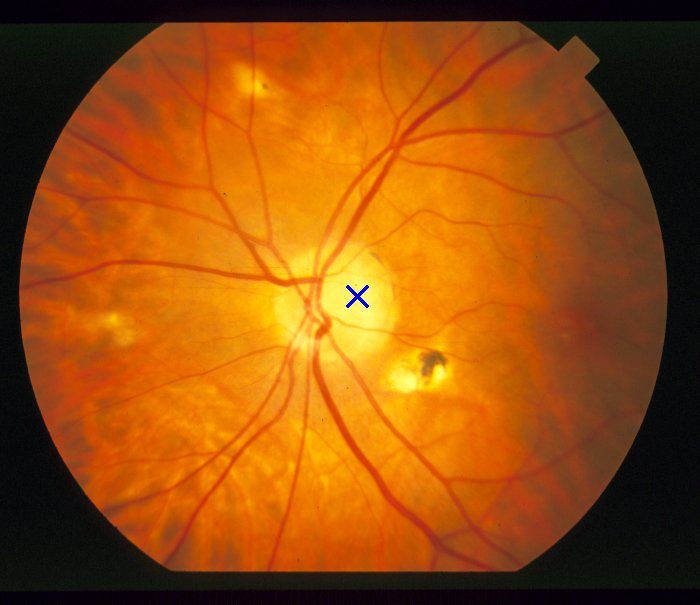
\includegraphics[width=3.0cm]{Images/Methode/Detection/Stare/im0183.jpg}{(k)} &
    	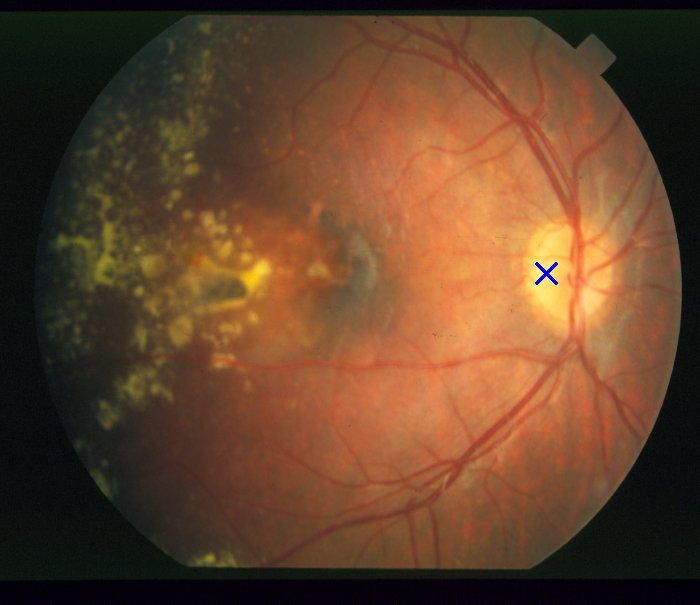
\includegraphics[width=3.0cm]{Images/Methode/Detection/Stare/im0177.jpg}{(l)} \\
    \end{tabular}

    
    \caption{\label{examples_detection}OD detection examples, in both healthy (1) and non-healthy (2) databases. The blue cross ($\times$) represents the found OD location point ((1) DRIVE database (six samples a, b, c, d, e, f), (2) STARE database (six samples g, h, i, j, k, l)).}
\end{figure*}

\begin{figure*}[!htbp]
    \centering

	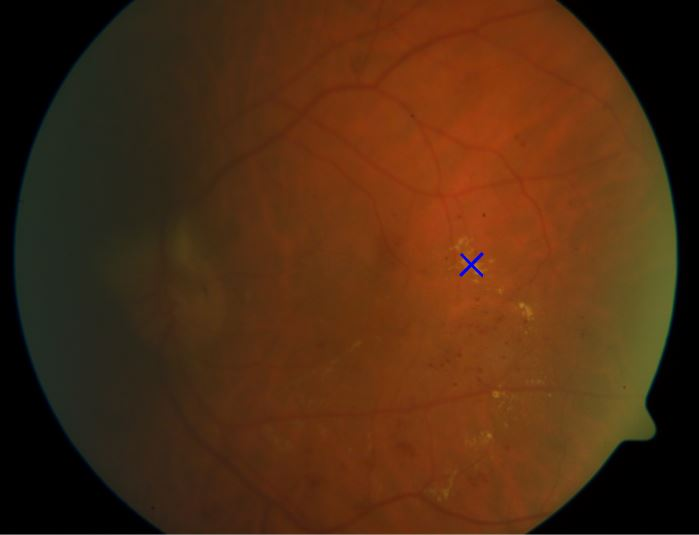
\includegraphics[height=2.7cm]{Images/Methode/Detection/failures/failure4.jpg}{(a)}
	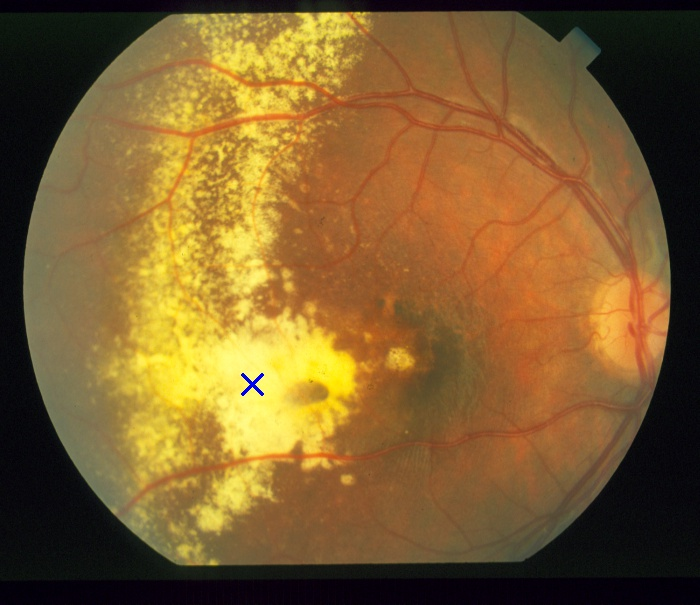
\includegraphics[height=2.7cm]{Images/Methode/Detection/failures/failure2.jpg}{(b)}
	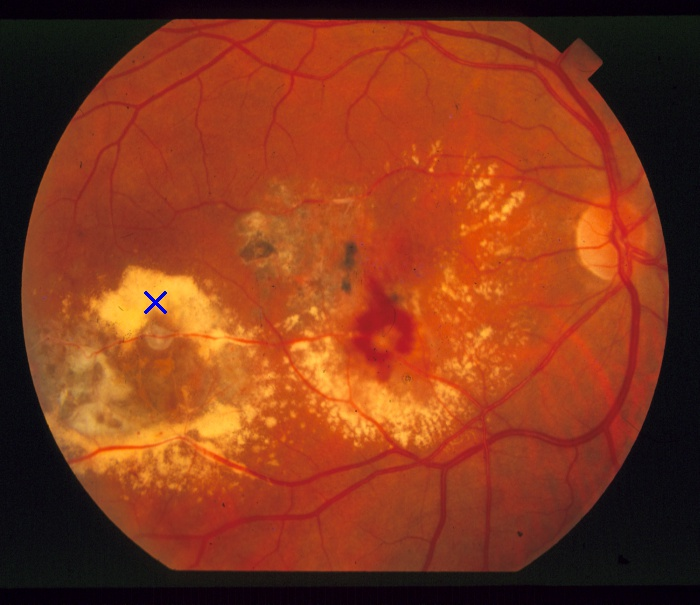
\includegraphics[height=2.7cm]{Images/Methode/Detection/failures/failure1.jpg}{(c)}
	
\caption{\label{examples_detection_failures} OD detection failures, in both healthy (a) and non-healthy (b, c) cases. The blue cross ($\times$) represents the found OD location point.}
\end{figure*}


\mbox{Fig. \ref{examples_detection}} presents a few qualitative results on OD detection, on both healthy (1) and pathological (2) retinal images. These results illustrate the ability to detect the OD, even in the presence of bright and spread lesions. In \mbox{Fig. \ref{examples_detection_failures}}, a few examples of OD detection failures are illustrated. In (a), a gradual darkening around the OD is observed, inducing a challenging detection using its brightness feature. In (b) and (c), large bright regions within the retina have resulted to a missing of the OD area, since the lesions are significantly brighter than the OD. Also, applying the template matching to find the final OD location may induce a wrong identification in rarer extreme cases.
The method for OD detection is applied on the different evaluation databases, and the obtained results are compared to the state-of-the-art methods. 
The proposed method achieves a 99.3\% detection rate on the different images from the evaluation databases.
In healthy retinal databases, where no bright lesions are apparent, such as VARIA, DRIVE, ROC or HRF, a 100\% detection is obtained. These results are equal or outperforms the state-of-the-art approaches for OD detection \citep{hashim,mahfouz,soares}. In pathological cases, where bright lesions are apparent, excellent performance on OD detection are also reached. Performance rates between 97.78\% and 99.49\% are obtained on these non-healthy databases, such as STARE, MESSIDOR, DIARETDB0, DIARETDB1, E-OPHTHA-EX or E-OPHTHA-MA. These results show the algorithm capacity to effectively detect the OD even in the presence of bright lesions, often having the same brightness feature as the disc. Globally, the method tends to outperform the state-of-the-art methods based on the brightness feature \citep{hashim,pourreza}, and compete with the methods based on the vascular tree extraction \citep{mahfouz,soares,zhang}, while ensuring a low complexity cost.

\subsubsection{OC and OD segmentation}

\begin{figure}[h]

    \centering
    \renewcommand{\arraystretch}{2}
    
    \begin{tabular}{c c c c c}
        
        {} & {(a)} & {(b)} & {(c)} & {(d)} \\
        {} & {} & {} & \multirow{2}{*}{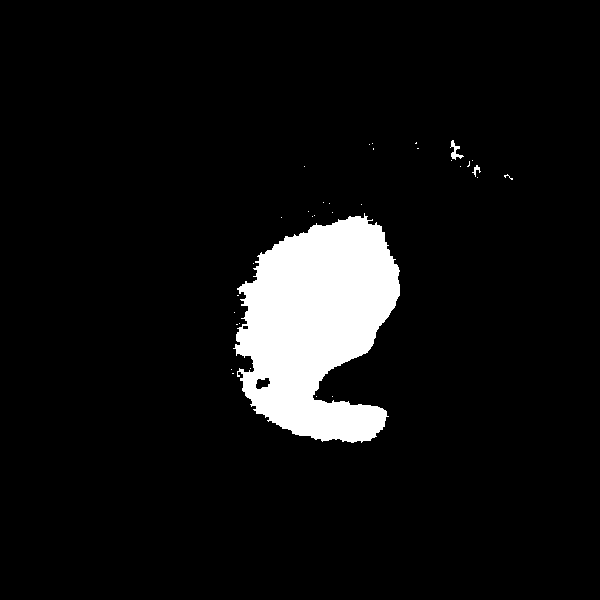
\includegraphics[width=2.5cm]{Images/Results/Segmentation/drishti98/2_cup.png}} & 
        \multirow{2}{*}{
\includegraphics[width=2.5cm]{Images/Results/Segmentation/drishti98/6_hough_cup.png}} \\
        
        {(1)} & \multirow{2}{*}{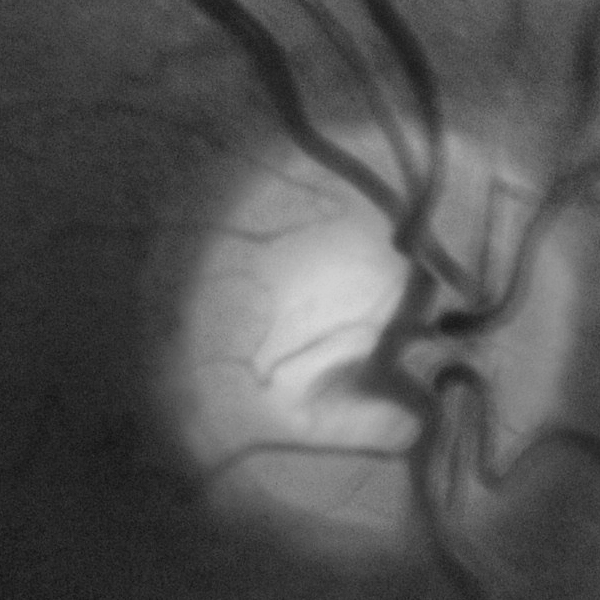
\includegraphics[width=2.5cm]{Images/Results/Segmentation/drishti98/0_crop.png}} & 
        \multirow{2}{*}{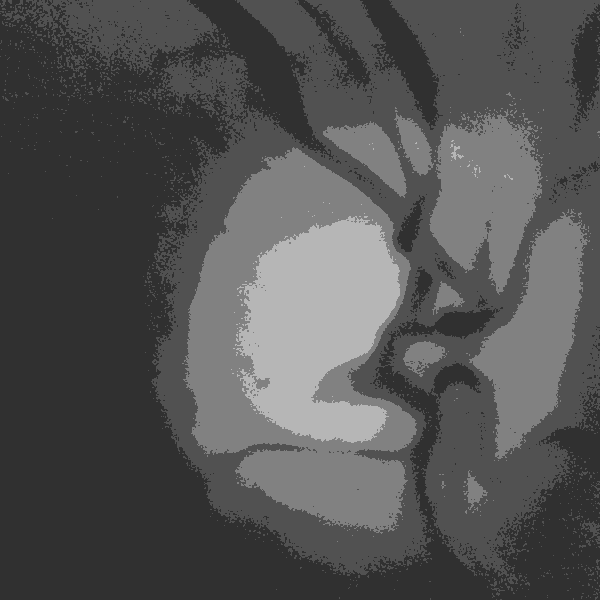
\includegraphics[width=2.5cm]{Images/Results/Segmentation/drishti98/1_kmeans.png}} & {} & {} \\
        
        {} & {} & {} & \multirow{2}{*}{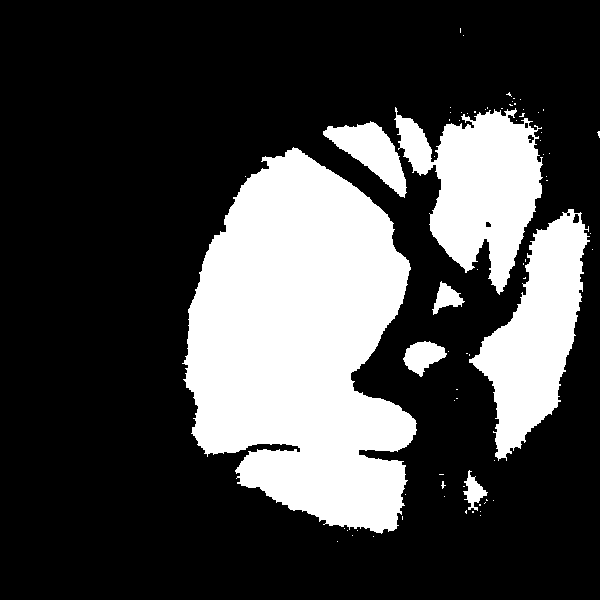
\includegraphics[width=2.5cm]{Images/Results/Segmentation/drishti98/3_do.png}} & 
        \multirow{2}{*}{
\includegraphics[width=2.5cm]{Images/Results/Segmentation/drishti98/7_hough_do.png}} \\
        
        {} & {} & {} & {} & {} \\
        {} & {} & {} & {} & {} \\
        
        {} & {} & {} & \multirow{2}{*}{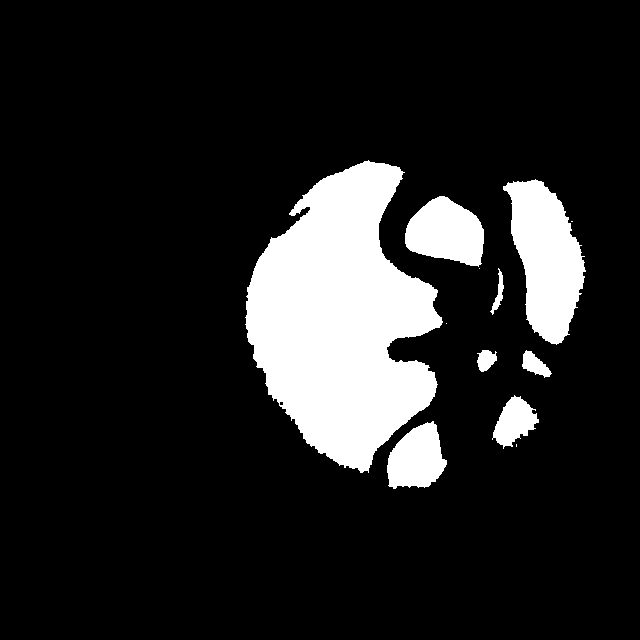
\includegraphics[width=2.5cm]{Images/Results/Segmentation/drishti69/2_cup.png}} & 
        \multirow{2}{*}{
\includegraphics[width=2.5cm]{Images/Results/Segmentation/drishti69/6_hough_cup.png}} \\
        
        {(2)} & \multirow{2}{*}{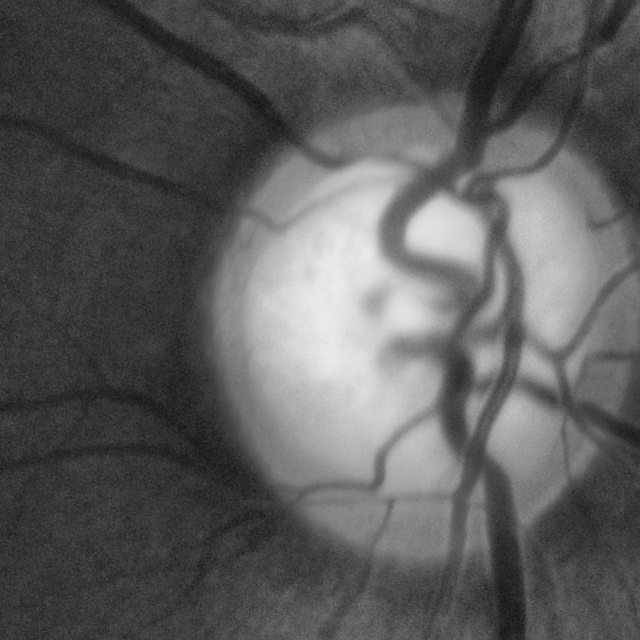
\includegraphics[width=2.5cm]{Images/Results/Segmentation/drishti69/0_crop.png}} & 
        \multirow{2}{*}{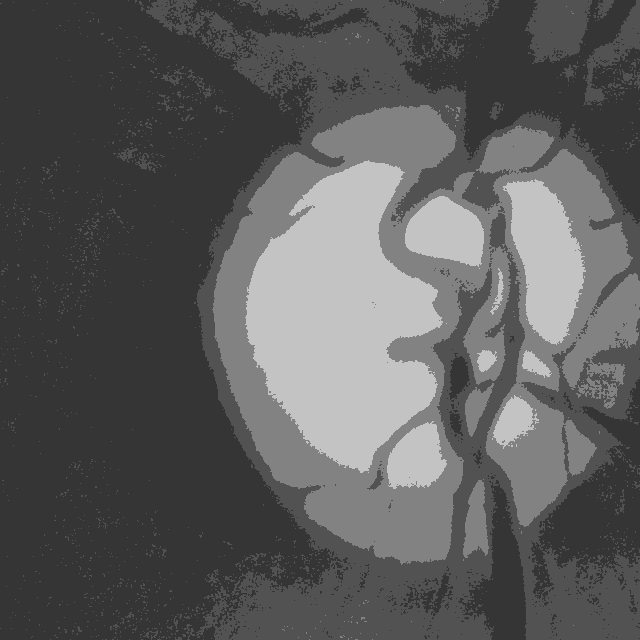
\includegraphics[width=2.5cm]{Images/Results/Segmentation/drishti69/1_kmeans.png}} & {} & {} \\
        
        {} & {} & {} & \multirow{2}{*}{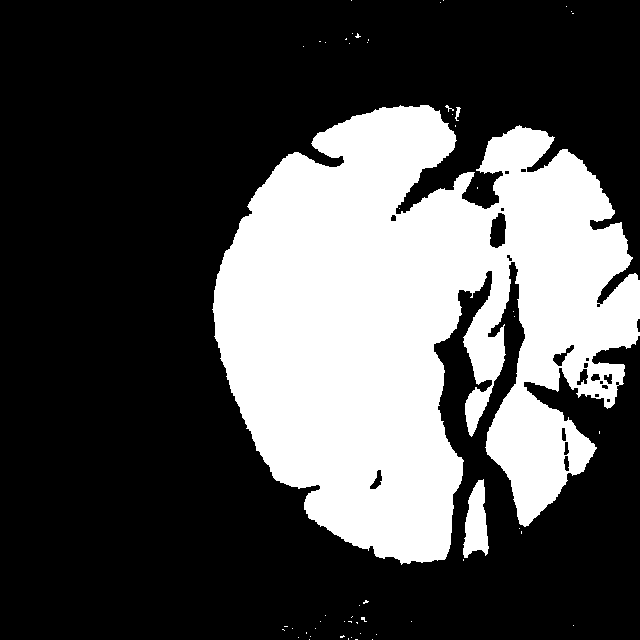
\includegraphics[width=2.5cm]{Images/Results/Segmentation/drishti69/3_do.png}} & 
        \multirow{2}{*}{
\includegraphics[width=2.5cm]{Images/Results/Segmentation/drishti69/7_hough_do.png}} \\
        
        {} & {} & {} & {} & {} \\

    \end{tabular}
    
    \caption{\label{segmentation_results}OC and OD segmentation examples, with healthy (1) and glaucomatous (2) images: (a) sub-image around the OD, (b) k-means clustering (K=4), (c) OC and OD extraction, (d) final segmentation with circular Hough transform.}
    
\end{figure}




Qualitative results for OC and OD segmentation are shown in \mbox{Fig. \ref{segmentation_results}}, illustrating the results for healthy (1) and glaucomatous (2) images from DRISHTI-GS1 database. A different cupping within the ONH is apparent between the two different examples. For each OD sub-image (a), we compute the K-means algorithm (b). Then, the clusters corresponding to the OC and OD areas are extracted (c). Finally, the circular Hough transform allows to find the boundaries of each area (d).

The DRISHTI-GS1 database was used to evaluate the performance of our segmentation method. A relevant ground-truth segmentation by four trained experts is provided for the OC and OD areas of each retinal image, both important for the ONH assessment. Hence, DRISHTI-GS1 is a well-used and pertinent database to benchmark different segmentation algorithms.
The proposed method for OC and OD segmentation was evaluated with the three sensitivity, PPV and F-score metrics (see Eq. (\ref{sensitivity}), (\ref{PPV}) and (\ref{fscore})). These metrics reflect the ability of the method to effectively classify the pixels belonging to the respective areas (OC and OD). 

For the sensitivity metric, 76.91\% and 83.05\% rates are obtained for the OC and OD areas respectively, testifying the encouraging performance of the segmentation method. 
For the PPV metric, excellent performance rates of 80.38\% and 94.32\% are respectively obtained for the OC and OD areas.
For the F-score metric, top-notch performance rates are reached by our proposed method, with a 79\% rate for the OC and a 91.45\% rate for the OD.

We also compare our results with the state-of-the-art methods, validated on DRISHTI-GS1 database. This comparison is made with the F-score metric, quantifying the region overlap between the computed area and the ground truth \citep{sivaswamy2014drishti}. The F-score brings a relevant measurement of the segmentation performance \citep{joshi}.
According to the F-score value, our method outperforms the method in \citet{cdr} with 77.1\% and compete with the method in \citet{cheng} reaching a 78.9\% rate. For the OD area, our method competes with the method in \citet{cdr} and \citet{cheng}, reaching 91.1\% and 92.1\% respectively.
These results show the ability of the algorithm to effectively purchase and classify each pixel belonging to the areas.

Globally, we notice that decreased rates are obtained for the OC area. It is due to the arduous task on effectively detect the borders, when the OC have not-well defined boundaries. It is the same case for the existing state-of-the-art methods.
Anyway, our segmentation stage achieves good performance and compete over the state-of-the-art methods, while using less complex algorithms. This precise segmentation allows a good approximation of the area-based CDR value for glaucoma screening.


\subsubsection{\label{glaucoma_screening_results}Glaucoma screening}

\begin{figure}[!htbp]
    \begin{minipage}{0.55\textwidth}
        \centering
        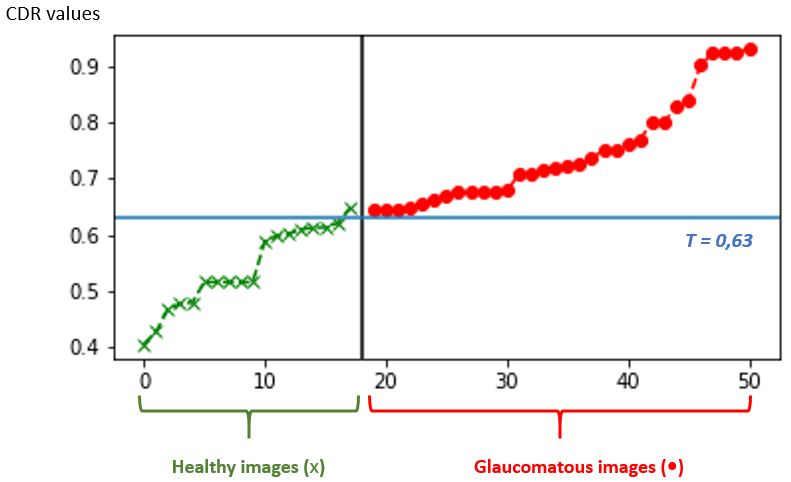
\includegraphics[width=0.9\textwidth]{Images/Results/Classification/ratio_legende.jpg}
        \captionof{figure}{\label{courbe_aire}CDR value for each retinal image, from healthy (green) class and glaucomatous (red) class (along x-axis: fifty annotated images from DRISHTI-GS1, along y-axis: CDR values (between 0 and 1)). The threshold value T = 0.63 is plotted in blue line along y-axis.}
    \end{minipage}
    \hfill
    \begin{minipage}{0.4\textwidth}
       \centering
       \begin{tabular}{|c|c|c|c|}
        \hline
        \multicolumn{2}{|c|}{Healthy class} & \multicolumn{2}{c|}{Glaucomatous class} \\
        \hline
        Mean & Standard & Mean & Standard  \\
        $\bar{m_H}$ & deviation & $\bar{m_G}$ & deviation \\
        {} & $\sigma_{H}$ & {} & $\sigma_{G}$ \\
        \hline
        0.541 & 0.07 & 0.74 & 0.09 \\
        \hline
        \end{tabular}
        \captionof{table}{\label{tableau_cdr_values}CDR mean and standard deviation values for healthy and glaucomatous classes.}
    \end{minipage}
\end{figure}

\begin{algorithm}[!htbp]

	\caption{Glaucoma screening}
	\label{alg:glaucomascreening}
	{\fontsize{10}{9}\selectfont
	\begin{algorithmic}[1]
		\State \textbf{Input:} OC segmentation $optic\_cup$, OD segmentation $optic\_disc$
		\State \textbf{Output:} Glaucoma diagnosis $diag$
		\medbreak
		
		\Function{glaucoma\_screening}{$optic\_cup, optic\_disc$}
		
		\State $area\_oc \gets$ \textsc{area\_calculation}$(optic\_cup)$
		\State $area\_od \gets$ \textsc{area\_calculation}$(optic\_disc)$
		\State $CDR \gets \frac{area\_oc}{area\_od}$
		\medbreak
		\If{$CDR > 0.63$}
			\State $diag \gets$ 'Glaucomatous'
		\Else
			\State $diag \gets$ 'Healthy'
		\EndIf
		\medbreak
		\State \textbf{return} $diag$
		\EndFunction
		
	\end{algorithmic}
	}
\end{algorithm}

\mbox{Fig. \ref{courbe_aire}} presents a graph with the computed $CDR_{area}$ value for each image from the annotated part of DRISHTI-GS1 database. Here, two distinct colors are apparent, according to the actual class of each retinal image: healthy images are represented in green color, when glaucomatous images are plotted in red color. 
Hence, CDR calculation finally leads to glaucoma screening and diagnosis. 
As explained in \mbox{section \ref{glaucoma_screening}} with the \mbox{Eq. (\ref{T})}, the threshold value $T$ is defined with the mean and standard deviation of each healthy and glaucomatous classes. \mbox{Table \ref{tableau_cdr_values}} presents the CDR mean value, as well as the standard deviation within each class. According to these values, the obtained threshold value $T = 0.63$ is also plotted in the graph, along the y-axis (see \mbox{Fig. \ref{courbe_aire}}). This threshold value $T$ is used to classify each image to its class (healthy or glaucomatous). 


\begin{figure}[t]

    \centering
	\renewcommand{\arraystretch}{0.8}
    
    \begin{tabular}{|c c c c c|}
    	
		\hline

		(a) & (b) & (c) & (d) & (e) \\
		
		\hline
		{} & {} & {} & {} & {} \\
		
		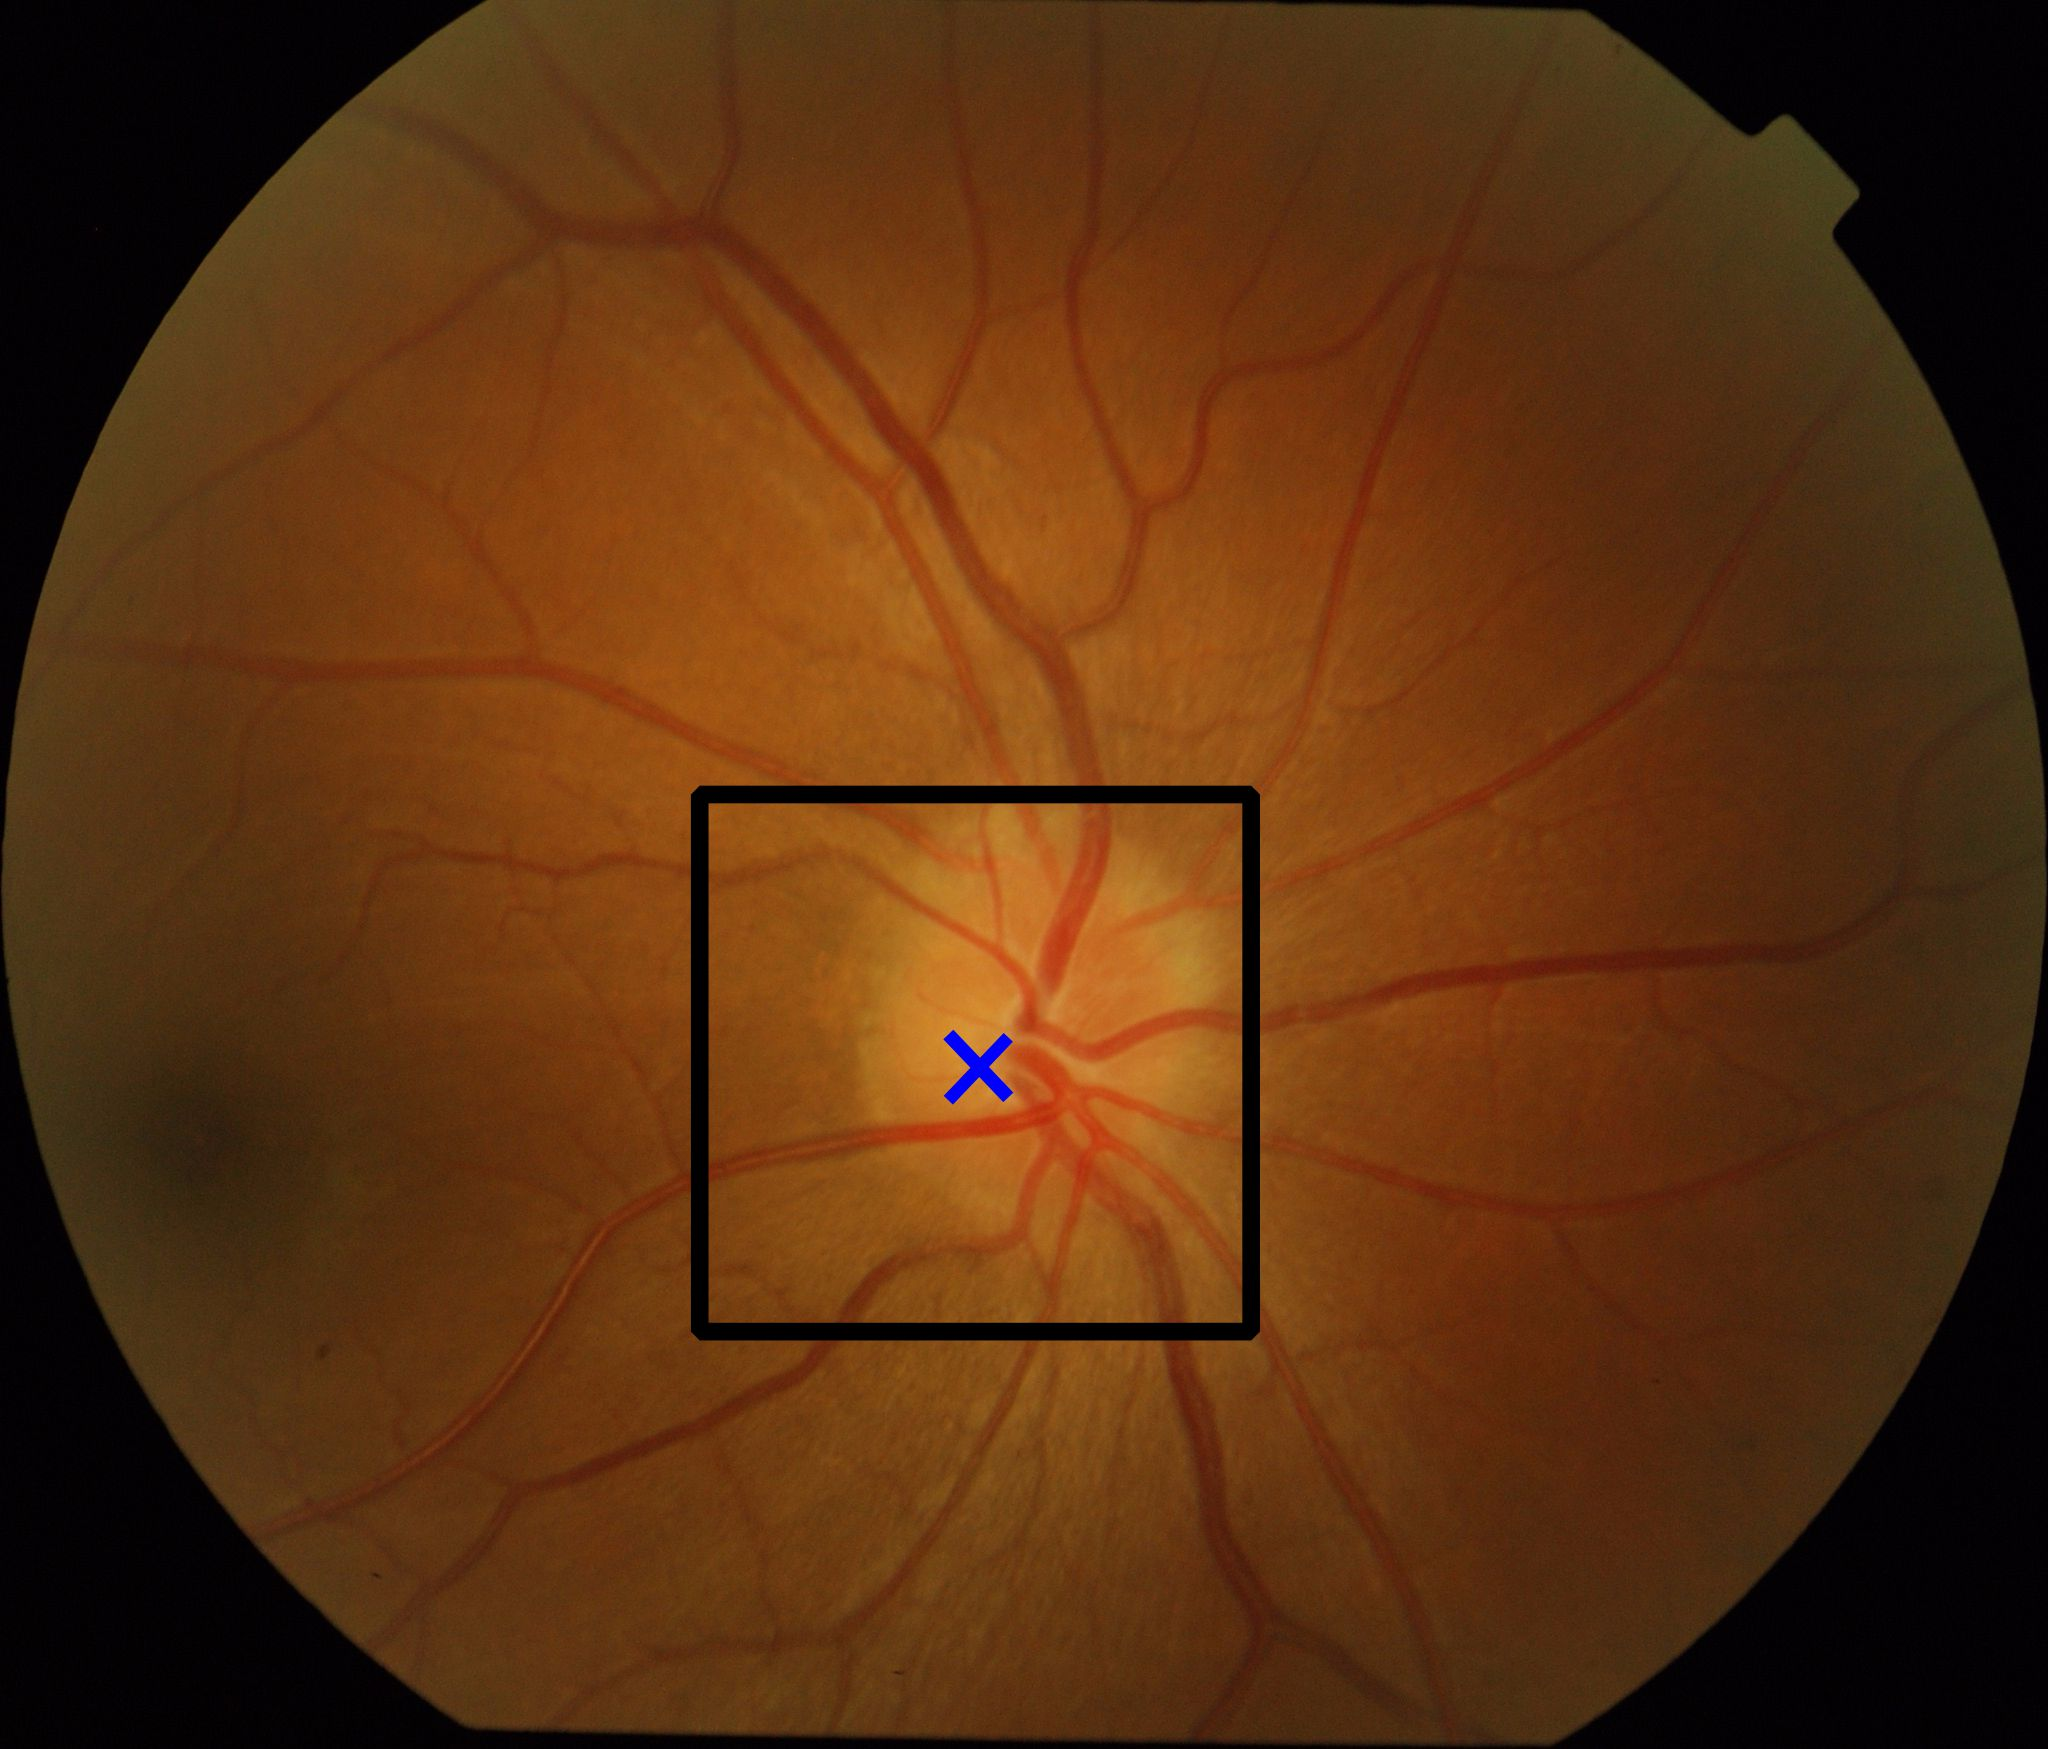
\includegraphics[width=3.5cm]{Images/Results/Segmentation/drishti101/od_detect.jpg} &
		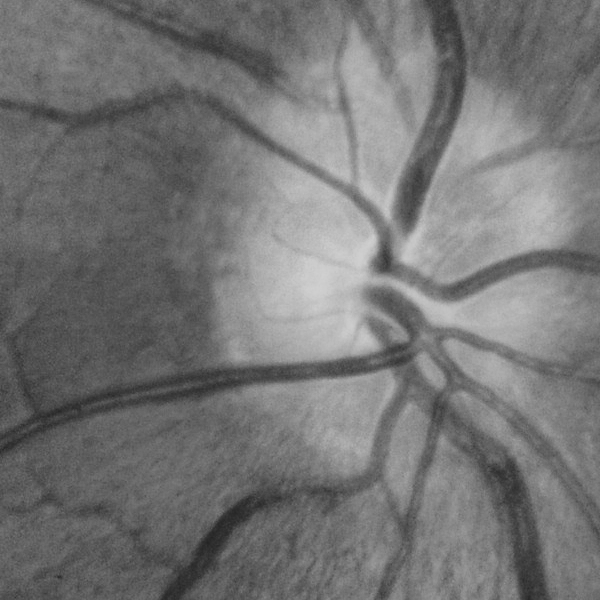
\includegraphics[width=3cm]{Images/Results/Segmentation/drishti101/0_crop.png} &
		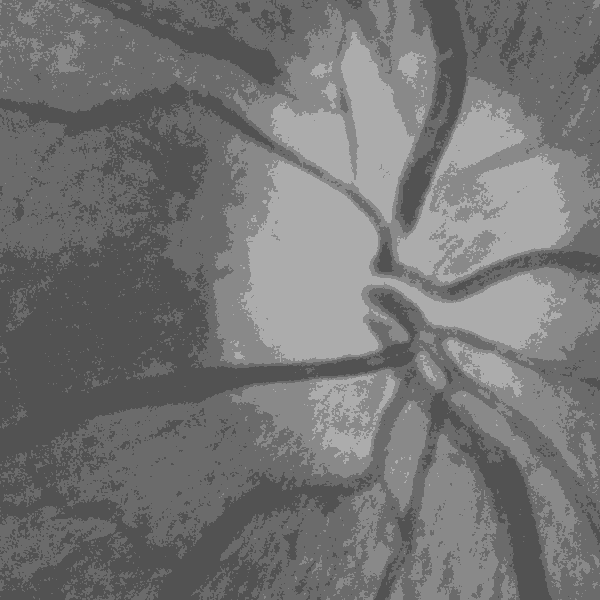
\includegraphics[width=3cm]{Images/Results/Segmentation/drishti101/1_kmeans.png} &
		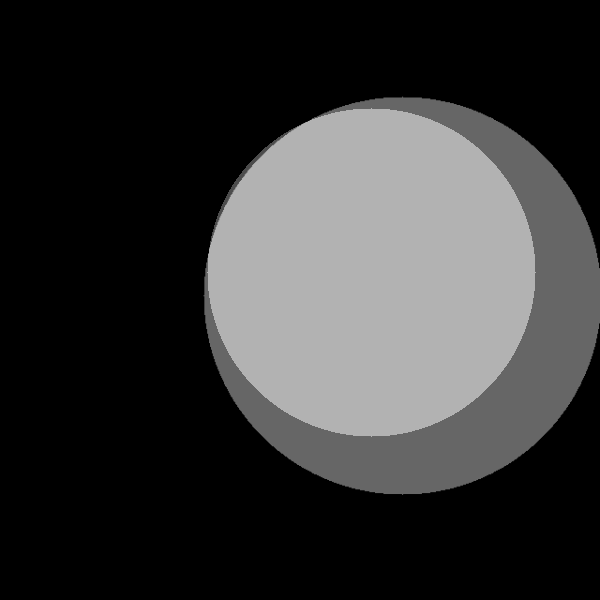
\includegraphics[width=3cm]{Images/Results/Segmentation/drishti101/overlay.png} &
		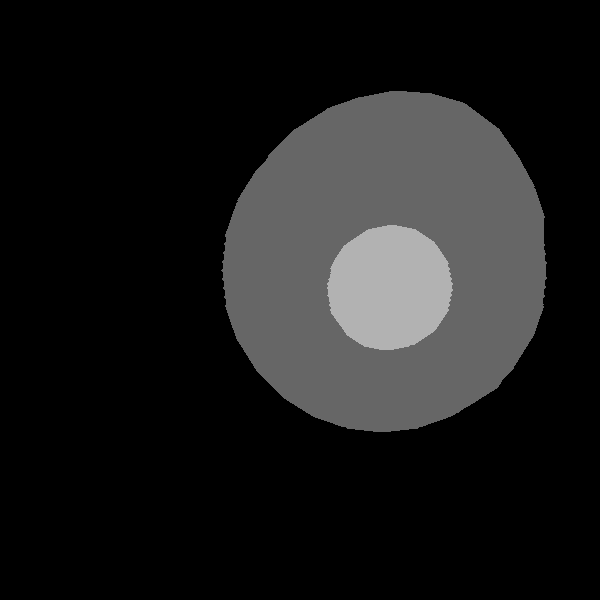
\includegraphics[width=3cm]{Images/Results/Segmentation/drishti101/overlay_gt.png} \\
		
		{} & {} & {} & CDR = 0.67 & CDR = 0.16 \\
		{} & {} & {} & $\updownarrow$ & $\updownarrow$ \\
		{} & {} & {} & Glaucomatous & Healthy \\
		
		\hline
    
    \end{tabular}

	\caption{\label{glaucoma_screening_failures}Glaucoma screening failure: (a) original retinal image, with OD location point (b) ROI extraction: sub-image around the OD, (c) k-means clustering (K=4), (d) joint OC-OD segmentation with CDR result and final diagnosis, (e) ground-truth joint OC-OD segmentation with CDR result and final diagnosis. The resulting segmentation leads to overestimated regions, and the CDR computation conducts to a false positive prediction.}

\end{figure}



\mbox{Fig. \ref{results}} shows some examples of the obtained results by our proposed method for glaucoma screening. Starting from each input image in the evaluation database, the OD is located (see \mbox{Fig \ref{results} (b)}) then extracted using the method for OD detection described in \mbox{section \ref{detection}}. \mbox{Fig \ref{results} (c)} shows this procedure. For the entire DRISHTI-GS1 database, an OD detection rate of 100\% is obtained, ensuring an efficient glaucoma screening process. 
Since the evaluation database is composed of healthy or glaucomatous images only, no bright lesions linked to other ocular diseases are apparent. However, the robust OD detection method is useful with eventual bright lesions, going with subjects suffering from other ocular diseases.
Then, our OC and OD segmentation method is performed using the approach described in \mbox{section \ref{segmentation}}. 
In \mbox{Fig. \ref{results} (d)}, the segmentation result is shown for OC and OD areas. Also, the ground-truth segmentation provided by the trained experts is exposed in \mbox{Fig. \ref{results} (e)}. Afterwards, the area-based CDR is computed, using the segmentation result. With the threshold value $T$ and the computed $CDR_{area}$ value for each retinal image, the binary classification is applied.
In \mbox{Fig. \ref{glaucoma_screening_failures}}, a failure in glaucoma screening is illustrated. Here, from the extracted sub-image around the OD (a), the OC and OD regions are segmented using the proposed method (b). Then, CDR computation leads to glaucoma screening using the defined threshold value. Here, since the boundaries of the regions of interest are difficult to define, overestimated OC and even OD regions are extracted. Hence, the computed segmentation affects the final result in glaucoma assessment, as the patient is wrongly diagnosed as suffering from glaucoma.


Following this, \mbox{Table \ref{classification_results}} exhibits the performance results, in comparison with some of the existing state-of-the-art methods for glaucoma screening.

\begin{table}[t]
\begin{center}
\small
\renewcommand{\arraystretch}{1.5}

 \begin{tabular}{|c|c|c|c|c|c|c|c|}
  \hline
  %{} & \multicolumn{2}{}{Supervised approaches} & \multicolumn{5}{}{Non-supervised approaches} \\
  Metric & \citeauthor{guerre} & \citeauthor{cdr} & \citeauthor{cheng} & \citeauthor{ayub} & \citeauthor{joshi} & \citeauthor{singh} & Proposed \\
  
  {} & \citeyearpar{guerre} & \citeyearpar{cdr} & \citeyearpar{cheng} & \citeyearpar{ayub} & \citeyearpar{joshi} & \citeyearpar{singh} & Method \\
  
  \hline
  
  Acc & 89 & 89.4 & 90.2 & 92 & 92.1 & 95 & \textbf{98} \\
  \hline
  Sen & 93 & 86.4 & 87.4 & 93 & 89.8 & \textbf{100} & \textbf{100} \\
  \hline
  Spe & 85 & 92.0 & 92.5 & 88 & 94.0 & 91 & \textbf{94.4} \\
  \hline
  PPV & 88 & - & - & - & - & 89 & \textbf{96.9} \\
  \hline
  NPV & 93 & - & - & - & - & \textbf{100} & \textbf{100} \\
  \hline
  F-Score & 90 & - & - & - & - & 94 & \textbf{98.4} \\
  \hline
 \end{tabular}
\caption{\label{classification_results}Obtained performance rates for glaucoma screening and diagnosis, in comparison with state-of-the art methods (\%).}
 \end{center}
 
 \end{table}


The proposed method achieves excellent results and improves the state-of-the-art methods on the performed metrics. An accuracy rate of 98\% on all the images is achieved, greater than the presented methods with performance rates between 89\% and 95\%. According to the accuracy rate and in accordance with the medical context, 98 subjects are well-diagnosed among 100 subjects with our proposed glaucoma screening method.
For the sensitivity metric, a 100\% rate is obtained, equal to the method in \citet{singh} and outperforming the other presented methods. That means that among 100 subjects actually suffering from glaucoma, the 100 subjects are detected as glaucomatous by the glaucoma screening system. This result strengthens the ability to effectively detect the glaucoma presence, in accordance with the motivations mentioned in \mbox{section \ref{metrics3}}.
For specificity, the proposed method reaches an excellent rate \mbox{of 94.4\%}, superior to the presented methods. Among 100 healthy subjects, more than 94 subjects are effectively consider as healthy by our glaucoma screening method. Less than 6 healthy subjects are considered as suffering from glaucoma, representing a false but non-serious alarm. 
For the PPV metric, our proposed method for glaucoma diagnosis obtains a 96.9\% rate, at \mbox{least 7.9\%} higher than the other approaches. This value highlights the system quality to properly classify an actual glaucomatous image, among all the images labeled as being affected by the disease. Also, for the NPV metric associated to the healthy class, a rate of 100\% equal to \citet{singh} method is reached, overriding the method in \citet{guerre}.
Finally, the F-score rate reaches the highest value with 98.4\%.
In accordance with the medical context in this work, this metric value highlights the system effectiveness on glaucoma labelling, while having well ability to find all actual glaucomatous images in the experimental sample.


\subsubsection{Computation time}

We implemented the proposed method for glaucoma screening on a Python environment with Anaconda, using an 3.3 GHz Intel Xeon CPU system with 8Gb of RAM. The computation time was evaluated in terms of average runtime for the images in DRISHTI-GS1 database. The prior and offline template creation is done \mbox{in 2.56 s}, allowing to construct the OD model for further OD detection. According to the online method for glaucoma screening, the first OD detection method (detection of bright regions, template matching) requires a computation time \mbox{of 8.31 s} per image. For OC and OD segmentation, the K-means clustering algorithm requires a computation time of 0.9 s. For the Hough transform, finding the boundary circle is made in an average time \mbox{of 2.08 s}. CDR calculation and glaucoma screening are almost instantaneous. Finally, the full-method is computed in \mbox{11 s}, showing off short computation time without any parallel optimization. This is in accordance with one of the purposes of this work formulated previously, as further implementation on portable platforms is intended.